\documentclass[a4paper]{article}

%=========================================
% Packages
%=========================================
\usepackage{mathtools}
\usepackage{amsfonts}
\usepackage{amsmath}
\usepackage{amssymb}
\usepackage{amsthm}
\usepackage[a4paper, total={6in, 8in}, margin=1in]{geometry}
\usepackage[utf8]{inputenc}
\usepackage{fancyhdr}
\usepackage[utf8]{inputenc}
\usepackage{graphicx}
\usepackage{physics}
\usepackage[listings]{tcolorbox}
\usepackage{hyperref}
\usepackage{tikz-cd}
\usepackage{adjustbox}
\usepackage{enumitem}
\usepackage[font=small,labelfont=bf]{caption}
\usepackage{subcaption}
\usepackage{wrapfig}
\usepackage{makecell}



\raggedright

\usetikzlibrary{arrows.meta}

\DeclarePairedDelimiter\ceil{\lceil}{\rceil}
\DeclarePairedDelimiter\floor{\lfloor}{\rfloor}

%=========================================
% Fonts
%=========================================
\usepackage{tgpagella}
\usepackage[T1]{fontenc}


%=========================================
% Custom Math Operators
%=========================================
\DeclareMathOperator{\adj}{adj}
\DeclareMathOperator{\im}{im}
\DeclareMathOperator{\nullity}{nullity}
\DeclareMathOperator{\sign}{sign}
\DeclareMathOperator{\dom}{dom}
\DeclareMathOperator{\lcm}{lcm}
\DeclareMathOperator{\ran}{ran}
\DeclareMathOperator{\ext}{Ext}
\DeclareMathOperator{\dist}{dist}
\DeclareMathOperator{\diam}{diam}
\DeclareMathOperator{\aut}{Aut}
\DeclareMathOperator{\inn}{Inn}
\DeclareMathOperator{\syl}{Syl}
\DeclareMathOperator{\edo}{End}
\DeclareMathOperator{\cov}{Cov}
\DeclareMathOperator{\vari}{Var}
\DeclareMathOperator{\cha}{char}
\DeclareMathOperator{\Span}{span}
\DeclareMathOperator{\ord}{ord}
\DeclareMathOperator{\res}{res}
\DeclareMathOperator{\Hom}{Hom}
\DeclareMathOperator{\Mor}{Mor}
\DeclareMathOperator{\coker}{coker}
\DeclareMathOperator{\Obj}{Obj}
\DeclareMathOperator{\id}{id}
\DeclareMathOperator{\GL}{GL}
\DeclareMathOperator*{\colim}{colim}

%=========================================
% Custom Commands (Shortcuts)
%=========================================
\newcommand{\CP}{\mathbb{CP}}
\newcommand{\GG}{\mathbb{G}}
\newcommand{\F}{\mathbb{F}}
\newcommand{\N}{\mathbb{N}}
\newcommand{\Q}{\mathbb{Q}}
\newcommand{\R}{\mathbb{R}}
\newcommand{\C}{\mathbb{C}}
\newcommand{\E}{\mathbb{E}}
\newcommand{\Prj}{\mathbb{P}}
\newcommand{\RP}{\mathbb{RP}}
\newcommand{\T}{\mathbb{T}}
\newcommand{\Z}{\mathbb{Z}}
\newcommand{\A}{\mathbb{A}}
\renewcommand{\H}{\mathbb{H}}
\newcommand{\K}{\mathbb{K}}

\newcommand{\mA}{\mathcal{A}}
\newcommand{\mB}{\mathcal{B}}
\newcommand{\mC}{\mathcal{C}}
\newcommand{\mD}{\mathcal{D}}
\newcommand{\mE}{\mathcal{E}}
\newcommand{\mF}{\mathcal{F}}
\newcommand{\mG}{\mathcal{G}}
\newcommand{\mH}{\mathcal{H}}
\newcommand{\mI}{\mathcal{I}}
\newcommand{\mJ}{\mathcal{J}}
\newcommand{\mK}{\mathcal{K}}
\newcommand{\mL}{\mathcal{L}}
\newcommand{\mM}{\mathcal{M}}
\newcommand{\mO}{\mathcal{O}}
\newcommand{\mP}{\mathcal{P}}
\newcommand{\mS}{\mathcal{S}}
\newcommand{\mT}{\mathcal{T}}
\newcommand{\mV}{\mathcal{V}}
\newcommand{\mW}{\mathcal{W}}

%=========================================
% Colours!!!
%=========================================
\definecolor{LightBlue}{HTML}{2D64A6}
\definecolor{ForestGreen}{HTML}{4BA150}
\definecolor{DarkBlue}{HTML}{000080}
\definecolor{LightPurple}{HTML}{cc99ff}
\definecolor{LightOrange}{HTML}{ffc34d}
\definecolor{Buff}{HTML}{DDAE7E}
\definecolor{Sunset}{HTML}{F2C57C}
\definecolor{Wenge}{HTML}{584B53}
\definecolor{Coolgray}{HTML}{9098CB}
\definecolor{Lavender}{HTML}{D6E3F8}
\definecolor{Glaucous}{HTML}{828BC4}
\definecolor{Mauve}{HTML}{C7A8F0}
\definecolor{Darkred}{HTML}{880808}
\definecolor{Beaver}{HTML}{9A8873}
\definecolor{UltraViolet}{HTML}{52489C}



%=========================================
% Theorem Environment
%=========================================
\tcbuselibrary{listings, theorems, breakable, skins}

\newtcbtheorem[number within = subsection]{thm}{Theorem}%
{	colback=Buff!3, 
	colframe=Buff, 
	fonttitle=\bfseries, 
	breakable, 
	enhanced jigsaw, 
	halign=left
}{thm}

\newtcbtheorem[number within=subsection, use counter from=thm]{defn}{Definition}%
{  colback=cyan!1,
    colframe=cyan!50!black,
	fonttitle=\bfseries, breakable, 
	enhanced jigsaw, 
	halign=left
}{defn}

\newtcbtheorem[number within=subsection, use counter from=thm]{axm}{Axiom}%
{	colback=red!5, 
	colframe=Darkred, 
	fonttitle=\bfseries, 
	breakable, 
	enhanced jigsaw, 
	halign=left
}{axm}

\newtcbtheorem[number within=subsection, use counter from=thm]{prp}{Proposition}%
{	colback=LightBlue!3, 
	colframe=Glaucous, 
	fonttitle=\bfseries, 
	breakable, 
	enhanced jigsaw, 
	halign=left
}{prp}

\newtcbtheorem[number within=subsection, use counter from=thm]{lmm}{Lemma}%
{	colback=LightBlue!3, 
	colframe=LightBlue!60, 
	fonttitle=\bfseries, 
	breakable, 
	enhanced jigsaw, 
	halign=left
}{lmm}

\newtcbtheorem[number within=subsection, use counter from=thm]{crl}{Corollary}%
{	colback=LightBlue!3, 
	colframe=LightBlue!60, 
	fonttitle=\bfseries, 
	breakable, 
	enhanced jigsaw, 
	halign=left
}{crl}

\newtcbtheorem[number within=subsection, use counter from=thm]{eg}{Example}%
{	colback=Beaver!5, 
	colframe=Beaver, 
	fonttitle=\bfseries, 
	breakable, 
	enhanced jigsaw, 
	halign=left
}{eg}

\newtcbtheorem[number within=subsection, use counter from=thm]{ex}{Exercise}%
{	colback=Beaver!5, 
	colframe=Beaver, 
	fonttitle=\bfseries, 
	breakable, 
	enhanced jigsaw, 
	halign=left
}{ex}

\newtcbtheorem[number within=subsection, use counter from=thm]{alg}{Algorithm}%
{	colback=UltraViolet!5, 
	colframe=UltraViolet, 
	fonttitle=\bfseries, 
	breakable, 
	enhanced jigsaw, 
	halign=left
}{alg}




%=========================================
% Hyperlinks
%=========================================
\hypersetup{
    colorlinks=true, %set true if you want colored links
    linktoc=all,     %set to all if you want both sections and subsections linked
    linkcolor=DarkBlue,  %choose some color if you want links to stand out
}


\pagestyle{fancy}
\fancyhf{}
\rhead{Labix}
\lhead{Algebraic Topology 3}
\rfoot{\thepage}

\title{Algebraic Topology 3}

\author{Labix}

\date{\today}
\begin{document}
\maketitle
\begin{abstract}
\begin{itemize}
\item Notes on Algebraic Topology by Oscar Randal-Williams
\end{itemize}
\end{abstract}
\pagebreak
\tableofcontents

\pagebreak

\section{Homotopy Theory}
\subsection{The nth Homotopy Groups}
\begin{defn}{Pairs of Space}{} Let $X$ be a topological space. A pair of space is a pair $(X,A)$ where $A\subseteq X$ is a subspace of $X$. A map of pairs $f:(X,A)\to(Y,B)$ is a continuous map $f:X\to Y$ such that $f(A)\subseteq B$. 
\end{defn}

\begin{defn}{Homotopy between Maps of Pairs}{} Let $f,g:(X,A)\to (Y,B)$ be maps of pairs. A homotopy between $f$ and $g$ is a homotopy $H:X\times[0,1]\to Y$ such that $H(A\times[0,1])\subseteq B$. 
\end{defn}

\begin{defn}{The nth Homotopy Groups}{} Let $(X,x_0)$ be a pointed space. Define the $n$th homotopy group $\pi_n(X,x_0)$ to be $$\pi_n(X,x_0)=\frac{\left\{f:\left(I^n,\partial I^n\right)\to\left(X,\{x_0\}\right)\;\bigg{|}\;f \text{ is continuous }\right\}}{\simeq}$$ where we say that $f\simeq g$ if there exists a homotopy between $f$ and $g$. 
\end{defn}

\begin{defn}{Concatenation}{} For $n\geq 1$, define a composition law on $\pi_n(X,x_0)$ for a pointed space $(X,x_0)$ by the formula $$(f\cdot g)(t_1,\dots,t_n)=\begin{cases}
f(2t_1,t_2,\dots,t_n) & \text{ if } 0\leq t_1\leq\frac{1}{2}\\
g(2t_1-1,t_2,\dots,t_n) & \text{ if } \frac{1}{2}\leq t\leq 1
\end{cases}$$ for $f,g\in\pi_n(X,x_0)$. 
\end{defn}

\begin{thm}{}{} Let $(X,x_0)$ be a pointed space and $n\geq 1$. The operation $\cdot$ on $\pi_n(X,x_0)$ is well defined and endows it with the structure of a group. 
\end{thm}

\begin{prp}{}{} Let $(X,x_0)$ be a pointed space. Then $\pi_n(X,x_0)$ is abelian for $n\geq 2$. 
\end{prp}

\subsection{Properties of Homotopy}
\begin{defn}{Category of Pointed Spaces}{} The Category of Pointed spaces $\text{Top}_\ast$ is defined where 
\begin{itemize}
\item The objects are pointed topological spaces $(X,x_0)$ for $x_0\in X$. 
\item The morphisms are continuous maps $f:X\to Y$ such that $f(x_0)=y_0$ for two pointed spaces $(X,x_0)$ and $(Y,y_0)$. 
\item Composition is defined as the composition of continuous maps that preserve the base point. 
\end{itemize}
\end{defn}

\begin{prp}{Functoriality}{} For each $n\geq 1$, $\pi_n(-):\text{Top}_\ast\to\text{Grp}$ is a functor where 
\begin{itemize}
\item On objects, it sends $(X,x_0)$ to the $n$th homotopy group $\pi_n(X,x_0)$
\item On morphisms, it sends $f:(X,x_0)\to (Y,y_0)$ to the induced map $$\pi_n(f):\pi_n(X,x_0)\to\pi_n(Y,y_0)$$ defined as $[\varphi]\mapsto[f\circ\varphi]$
\end{itemize}
\end{prp}

\begin{prp}{}{} Let $(X,x_0),(Y,y_0)$ be pointed spaces and $f,g:(X,x_0)\to (Y,y_0)$ be pointed maps. If $f$ and $g$ are homotopic, then the induced maps $$\pi_n(f)=\pi_n(g):\pi_n(X,x_0)\to\pi_n(Y,y_0)$$ are equal. Moreover, if $f$ is a homotopy equivalence, then $\pi_n(f)$ is an isomorphism. 
\end{prp}

\begin{thm}{}{} Let $(X,x_0)$ and $(X,x_1)$ be pointed spaces with the same base space. If $u:I\to X$ is a path from $x_0$ to $x_1$, then $u$ induces a map $$u_\#:\pi_n(X,x_1)\to\pi_n(X,x_0)$$ satisfying the following functorial properties: 
\begin{itemize}
\item $u_\#$ is a group homomorphism
\item If $v:I\to X$ is a path from $x_1$ to $x_2$ and $u\cdot v$ is the concatenation of these paths, then $$(u\cdot v)_\#=u_\#\circ v_\#$$
\item If $c_{x_0}$ is the constant path from $x_0$ to $x_0$ then $(c_{x_0})_\#$ is the identity
\end{itemize}
\end{thm}

\begin{prp}{}{} Let $(X,x_0)$ and $(X,x_1)$ be pointed spaces with the same base space. Let $u,v:I\to X$ be paths from $x_0$ to $x_1$. If $u$ and $v$ are homotopic relative to end points then the induced maps $$u_\#=v_\#:\pi_n(X,x_1)\to\pi_n(X,x_0)$$ are equal. 
\end{prp}

\begin{crl}{}{} Let $(X,x_0)$ and $(X,x_1)$ be pointed spaces with the same base space. If $x_0$ and $x_1$ are path connected, then $$\pi_n(X,x_0)\cong\pi_n(X,x_1)$$ where the isomorphism depends on the choice of path from $x_0$ to $x_1$. 
\end{crl}

\begin{prp}{}{} Let $(X,x_0)$ be a pointed space and $f\in\pi_n(X,x_0)$. Let $u:I\to X$ be a loop on $x_0$. Then $u$ induces a left action of $\pi_1(X,x_0)$ on $\pi_n(X,x_0)$ by the map $$(u,f)\mapsto u_\#(f)=u\cdot f\cdot u^{-1}$$ In particular, for $n\geq 2$, $\pi_n(X,x_0)$ is a $\Z\pi_1(X,x_0)$-module. 
\end{prp}

\subsection{Relative Homotopy Groups}
\begin{defn}{Triplets of Spaces}{} Let $X$ be a topological space. A pointed pair of space is a triple $(X,A_1,A_2)$ where $A_2\subseteq A_1\subseteq X$ are subspaces of $X$. A map between triplets of spaces $f:(X,A_1,A_2)\to(Y,B_1,B_2)$ is a map $f:X\to Y$ such that $f(A_1)\subseteq B_1$ and $f(A_2)\subseteq B_2$. \\~\\
If $A_2=\{x_0\}$ is a single point we say that $(X,A,x_0)$ is a pointed pair of spaces. 
\end{defn}

\begin{defn}{Homotopy between Maps of Triplets}{} Let $f,g:(X,A_1,A_2)\to(Y,B_1,B_2)$ be maps triplets of spaces. A homotopy between $f$ and $g$ is a homotopy between $f:X\to Y$ and $g:X\to Y$, namely $H:X\times[0,1]\to Y$ such that $H(A_1\times[0,1])\subseteq B_1$ and $H(A_2\times[0,1])\subseteq B_2$. 
\end{defn}

For a pointed pair of spaces $(X,A,x_0)$, the inclusion $\iota:(A,x_0)\to(X,x_0)$ induces a map on homotopy $$\pi_n(\iota)=\pi_n(A,x_0)\to\pi_n(X,x_0)$$ which is in general not injective. For $[\alpha]\in\pi_n(A,x_0)$ to lie in the kernel, it must satisfy that for any map $f:(I,\partial I^n)\to(A,x_0)$ representing $[\alpha]$, $\iota\circ f$ is homotopic to the constant map $c_{x_0}$ on $x_0$. Such a homotopy is a map $H:I^n\times I\to X$ satisfying the following conditions: 
\begin{itemize}
\item $H(-,1)=f$
\item $H(-,0)=c_{x_0}$
\item $H|_{\partial I^n\times I}=c_{x_0}$
\end{itemize}
Thus if we denote $$J^n=I^n\times\{0\}\cup\partial I^n\times I$$ which is a subspace of the boundary $\partial I^{n+1}$, such a homotopy $H$ is a map of triplets of spaces $$H:(I^{n+1},\partial I^n,J^n)\to(X,A,x_0)$$

\begin{defn}{The nth Relative Homotopy Groups}{} Let $(X,A,x_0)$ be a pointed pair of space. Define the relative homotopy groups of the triple by $$\pi_n(X,A,x_0)=\frac{\left\{f:\left(I^n,\partial I^n,J^{n-1}\right)\to\left(X,A,\{x_0\}\right)\;\bigg{|}\;f \text{ is continuous }\right\}}{\simeq}$$ for $n\geq 2$, where $J^n=I^n\times\{0\}\cup\partial I^n\times I$ and we say that $f\simeq g$ if there exists a homotopy between $f$ and $g$. 
\end{defn}

\begin{thm}{}{} Let $(X,A,x_0)$ be a pointed pair of space. The composition law on definition 1.1.4 defines a group structure on $\pi_n(X,A,x_0)$ for $n\geq 2$. 
\end{thm}

\begin{crl}{}{} Let $(X,A,x_0)$ be a pointed pair of space. For $n\geq 3$, $\pi_n(X,A,x_0)$ is abelian. 
\end{crl}

\subsection{Induced Maps of Relative Homotopy Groups}
\begin{thm}{}{} Let $(X,A,x_0)$ and $(Y,B,y_0)$ be pointed pairs of spaces and $f:(X,A,x_0)\to(Y,B,y_0)$ a map. Then $f$ induces a map on the relative homotopy groups $$f_\ast:\pi_n(X,A,x_0)\to\pi_n(Y,B,y_0)$$ for $n\geq 2$ satisfying the following functorial properties: 
\begin{itemize}
\item $f_\ast$ is a group homomorphism
\item If $g:(Y,B,y_0)\to(Z,C,z_0)$ is a map, then $$(g\circ f)_\ast=g_\ast\circ f_\ast$$
\item If $\text{id}_{(X,A,x_0)}$ is the identity map on $(X,A,x_0)$, then $$(\text{id}_{(X,A,x_0)})_\ast=\text{id}_{\pi_n(X,A,x_0)}$$
\end{itemize}
\end{thm}

\begin{prp}{}{} Let $(X,A,x_0),(Y,B,y_0)$ be pointed pairs of spaces and $f,g:(X,A,x_0)\to (Y,B,y_0)$ be pointed maps. If $f$ and $g$ are homotopic, then the induced maps $$f_\ast=g_\ast:\pi_n(X,A,x_0)\to\pi_n(Y,B,y_0)$$ are equal. Moreover, if $f$ is a homotopy equivalence, then $f_\ast$ is an isomorphism. 
\end{prp}

\begin{prp}{}{} The relative homotopy groups of $(X,A,x_0)$ fit into a long exact sequence \\~\\
\adjustbox{scale=0.75,center}{\begin{tikzcd}
	\cdots & {\pi_{n+1}(X,A,x_0)} & {\pi_n(A,x_0)} & {\pi_n(X,x_0)} & {\pi_n(X,A,x_0)} & {\pi_{n-1}(A,x_0)} & \cdots & {\pi_0(X,x_0)} & 0
	\arrow[from=1-1, to=1-2]
	\arrow["{\partial_{n+1}}", from=1-2, to=1-3]
	\arrow["{i_\ast}", from=1-3, to=1-4]
	\arrow["{j_\ast}", from=1-4, to=1-5]
	\arrow["{\partial_n}", from=1-5, to=1-6]
	\arrow[from=1-6, to=1-7]
	\arrow[from=1-8, to=1-9]
	\arrow[from=1-7, to=1-8]
\end{tikzcd}}\\~\\
where $\partial_n$ is defined by $[f]\mapsto [f|_{I^{n-1}}]$ and $i_\ast$ and $j_\ast$ are induced by inclusions. 
\end{prp}

Note that even though at the end of the sequence group structures are not defined, exactness still makes sense: kernels in this case consists of elements that map to the homotopy class of the constant map. 

\begin{thm}{The Hurewicz Homomorphism}{} Let $(X,A,x_0)$ be a pointed pair of space. Let $u_n$ be a generator of $H_n(S^n)\cong\Z$. Then the map $$h:\pi_n(X,A,x_0)\to H_n(X,A)$$ defined by $[f]\mapsto f_\ast(u_n)$ is a group homomorphism. 
\end{thm}

\subsection{n-Connectedness}
\begin{defn}{n-Connected Space}{} We say that the pair $(X,A)$ is $n$-connected if $\pi_i(X,A)=0$ for $i\leq n$ and $X$ is $n$-connected if $\pi_i(X)=0$ for $i\leq n$. 
\end{defn}

\subsection{Weakly Contractible Space}
\begin{defn}{Weakly Contractible}{} Let $X$ be a space. We say that $X$ is weakly contractible if $$\pi_n(X)=0$$ for all $n\geq 0$. 
\end{defn}

\pagebreak
\section{Homotopy and CW-Complexes}
\subsection{Whitehead's Theorem}
\begin{defn}{Weak Homotopy Equivalence}{} We say that a map $f:X\to Y$ is a weak homotopy equivalence if it induces isomorphisms on all homotopy groups $\pi_n$ on any choice of base point. 
\end{defn}

\begin{thm}{Whitehead's Theorem}{} If $X$ and $Y$ are CW-complexes and $f:X\to Y$ is a weak homotopy equivalence, then $f$ is a homotopy equivalence. 
\end{thm}

\begin{crl}{}{} If $X$ and $Y$ are CW-complexes with $\pi_1(X)=\pi_1(Y)=0$ and $f:X\to Y$ induces isomorphisms on homology groups $H_n$ for all $n$, then $f$ is a homotopy equivalence. 
\end{crl}

\subsection{Cellular Approximations}
\begin{defn}{Cellular Maps}{} Let $X$ and $Y$ be CW-complexes. A map $f:X\to Y$ is called cellular if $f(X_n)\subset Y_n$ for all $n$, where $X_n$ is the $n$-skeleton of $X$. 
\end{defn}

\begin{defn}{Cellular Approximations}{} Let $X$ and $Y$ be CW-complexes. We say that $f:X\to Y$ has a cellular approximations if $f$ is homotopic to a cellular map $f':X\to Y$. 
\end{defn}

\begin{thm}{Cellular Approximation Theorem}{} Any map $f:X\to Y$ between CW-complexes has a cellular approximation $f':X\to Y$. Moreover, if $f$ is already cellular on a subcomplex $A\subseteq X$, then we can take $f'|_A=f|_A$. 
\end{thm}

\begin{thm}{Relative Cellular Approximation}{} Any map $f:(X,A)\to (Y,B)$ between pairs of CW-complexes has a cellular approximation. 
\end{thm}

\begin{crl}{}{} Let $A\subset X$ be CW-complexes and suppose that all cells $X\setminus A$ have dimension larger than $n$. Then $\pi_i(X,A)=0$ for all $i\leq n$. 
\end{crl}

\begin{crl}{}{} If $X$ is a CW-complex, then $\pi_i(X,X_n)=0$ for all $i\leq n$. 
\end{crl}

\begin{crl}{}{} Let $X$ be a CW-complex. Then $$\pi(X)\cong\pi(X_n)$$ for $i<n$. 
\end{crl}

\subsection{CW Approximations}
\begin{defn}{CW Approximation}{} A CW approximation of $X$ is a weak homotopy equivalence $f:Z\to X$ where $Z$ is a CW approximation. 
\end{defn}


\begin{defn}{CW Model}{} Let $(X,A)$ be a non-empty pair of CW-complexes. An $n$-connected CW model of $(X,A)$ is an $n$-connected CW pair $(Z,A)$ together with a map $f:Z\to X$ with $f|_A=\text{id}_A$ such that $$f_\ast:\pi_i(Z)\to\pi_i(X)$$ is an isomorphism for $i>n$ and an injection for $i=n$ for any choice of base point. 
\end{defn}

\begin{thm}{}{} For any non-empty pair $(X,A)$ of CW-complexes, there exists an $n$-connected model $(Z,A)$. Moreover, $Z$ can be built from $A$ by attaching cells of dimension greater than $n$. 
\end{thm}

\begin{crl}{}{} Every pair of CW-complex $(X,A)$ has a CW approximation $(Z,B)$. 
\end{crl}

Thus we have shown existence of CW approximations, it remains to show uniqueness. 

\begin{crl}{}{} CW-approximations are unique up to homotopy equivalence. 
\end{crl}

\pagebreak

\section{Main Results of Homotopy Theory on CW-Complexes}
\subsection{Excision for Homotopy Groups}
\begin{thm}{The Homotopy Excision Theorem}{} Let $X$ be a CW-complex decomposed as the union of subcomplexes $A$ and $B$ with non-empty connected intersection $C=A\cap B$. If $(A,C)$ is $m$-connected and $(B,C)$ is $n$-connected for $m,n\geq 0$, then the map $$\iota_\ast:\pi_i(A,C)\to(X,B)$$ induced by the inclusion $\iota:(A,C)\to(X,B)$ is an isomorphism for $i<m+n$ and a surjection for $i=m+n$. 
\end{thm}

\subsection{Freudenthal Suspension Theorem}
\begin{defn}{Reduced Suspension}{} Let $(X,x_0)$ be a pointed space. Define the reduced suspension of $X$ to be the space $$\Sigma X=\frac{X\times I}{(X\times\{0\}\cup X\times\{1\}\cup\{x_0\}\times I)}$$
\end{defn}

The reduced suspension defines a continuous map sending a space $X$ to its reduced suspension $\Sigma X$. 

\begin{thm}{Freudenthal Suspension Theorem}{} Let $X$ be an $(n-1)$-connected CW complex. Then for $0\leq k\leq 2n-2$, the induced map $$\Sigma_\ast:\pi_k(X)\to\pi_{k+1}(\Sigma X)$$ is an isomorphism. For $k=2n-1$, $\Sigma_\ast$ is a surjection. 
\end{thm}

\begin{crl}{}{} Let $n\geq 0$. Then there is an isomorphism $$\pi_n(S^n)\cong\pi_{n+1}(S^{n+1})$$
\end{crl}

\begin{defn}{Stable Homotopy Groups}{} Let $X$ be a space. Let $n\in\N$. Define the $n$th stable homotopy groups of $X$ to be $$\pi_n^s(X)=\colim_{k\to\infty}\pi_{n+k}(\Sigma^kX)$$
\end{defn}

\subsection{Hurewicz's Theorem}
\begin{thm}{Hurewicz's Theorem}{} Let $X$ be a $(n-1)$-connected space and $n\geq 2$. Then $\widetilde{H}_i(X)=0$ for all $i<n$ and $\pi_n(X)\cong H_n(X)$. \\~\\

Moreover, if a pair $(X,A)$ is $(n-1)$-connected with $n\geq 2$ and $\pi_1(A)=0$, then $H_i(X,A)=0$ for all $i<n$ and $\pi_n(X,A)\cong H_n(X,A)$
\end{thm}

\subsection{Eilenberg-MacLane Spaces}
\begin{defn}{Eilenberg-MacLane Space}{} Let $G$ be a group and $n\in\N$. We say that a space $X$ is an Eilenberg-MacLane space of type $K(G,n)$ if $\pi_n(X)=G$ and $\pi_k(X)=0$ for all $k\neq n$. 
\end{defn}

\begin{prp}{}{} Let $G$ be a group. Then there exists a $K(G,1)$-CW complex. 
\end{prp}

\begin{thm}{}{} Let $G$ be an abelian group and $n\geq 2$. Then there exists a $K(G,n)$-CW complex. 
\end{thm}

\begin{thm}{}{} Let $X$ be a space. Then there is a natural bijection $$H^n(X;G)\cong[X,K(G,n)]$$ 
\end{thm}

\begin{thm}{}{} Let $X$ be a CW complex. Let $G$ be an abelian group. Let $n\in\N$. Then there is a natural isomorphism $$\widetilde{H}_k(X;G)\cong\colim_{n\to\infty}\pi_{k+n}(X\wedge K(G,n))$$
\end{thm}

\pagebreak
\section{Generalized Homology and Cohomology Theories}
\subsection{Homology Theories}
\begin{defn}{The Category of Pairs of CW Complexes}{} Define the category of CW pairs $\bold{CW}^2$ to be the category where objects are pairs $(X,A)$ of CW complexes where $A\subseteq X$, and the morphisms are maps of pairs. 
\end{defn}

\begin{defn}{Generalized Homology Theory for CW Pairs}{} A Generalized Homology Theory is a collection of functors and natural transformations $$h_n:\bold{CW}^2\to\bold{Ab}\;\;\;\;\;\;\;\text{ and }\;\;\;\;\;\;\;\delta_n:h_n(X,Y)\to h_{n-1}(Y,\emptyset)$$ satisfying the following. 
\begin{itemize}
\item Homotopy Invariance: If $f\simeq g:(X,A)\to(Y,B)$ then $$h_n(f)=h_n(g):h_n(X,A)\to h_n(Y,B)$$
\item Exactness: There exists a short exact sequence \\~\\
\adjustbox{scale=1.0,center}{\begin{tikzcd}
	\cdots & {h_{n+1}(X,A)} & {h_n(A)} & {h_n(X)} & {h_n(X,A)} & {h_{n-1}(A)} & \cdots
	\arrow[from=1-1, to=1-2]
	\arrow["{\delta_{n+1}}", from=1-2, to=1-3]
	\arrow[from=1-3, to=1-4]
	\arrow[from=1-4, to=1-5]
	\arrow["{\delta_n}", from=1-5, to=1-6]
	\arrow[from=1-6, to=1-7]
\end{tikzcd}}~\\
\item Additivity: If $(X,A)=\coprod_{i\in I}(X_i,A_i)$, then the direct sum of the inclusion maps $$\bigoplus_{i\in I}h_n(X_i,A_i)\cong h_n(X,A)$$ is an isomorphism
\item Excision: If $\overline{E}\subseteq A^\circ\subseteq X$, then $$h_n(X\setminus E,A\setminus E)\cong h_n(X,A)$$ induced by the inclusion map
\end{itemize}
\end{defn}

We mention for once and for all that the additivity axiom is required only when the CW complexes are finite. In particular, in order for the homology theory to be meaningful, we must restrict the underlying category of spaces to be finite CW complexes if one drops the additivity axiom. 

\begin{lmm}{}{} The excision axiom is equivalent to saying that $X=A^\circ\cup B^\circ$ with inclusion map $\iota:(B,A\cap B)\to (X,A)$ implies $h_n(\iota):h_n(B,A\cap B)\to h_n(X,A)$ is an isomorphism. 
\end{lmm}

\begin{defn}{The Category of Pairs of Spaces}{} Define the category of CW pairs $\bold{Top}^2$ to be the category where objects are pairs $(X,Y)$ of spaces, and the morphisms are maps of pairs. 
\end{defn}

\begin{defn}{Generalized Homology Theory}{} A Generalized Homology Theory is a collection of functors $$h_n:\bold{Top}^2\to\bold{Ab}\;\;\;\;\;\;\;\text{ and }\;\;\;\;\;\;\;\delta_n:h_n(X,Y)\to h_{n-1}(Y,\emptyset)$$ satisfying the firs four axioms together with the following. 
\begin{itemize}
\item Weak Equivalence: If $f:(X,A)\to(Y,B)$ is a weak equivalence, then $$f_\ast:h_n(X,A)\to h_n(Y,B)$$ is an isomorphism. 
\end{itemize}
\end{defn}

By adding on the axiom of weak equivalence and the fact that every space admits a weak equivalence to a CW complex, we can see that the two theories are the same. However, note that in this case some of the working homology theories are not a generalized homology theory in this sense (when we encounter the dual notion, sheaf cohomology is not a generalized cohomology theory). 

\begin{thm}{}{} Any generalized homology theory on $\bold{Top}^2$ determines and is determined by a generalized homology theory on $\bold{CW}^2$.
\end{thm}

\begin{defn}{Homology Theory}{} If a generalized homology theory $(h_n,\delta_n)$ in addition satisfies 
\begin{itemize}
\item Dimension: $$h_n(\ast)=\begin{cases}
\Z & \text{ if } n=0\\
0 & \text{ otherwise }
\end{cases}$$
\end{itemize}
Then $h_n$ is called a homology theory. 
\end{defn}

The same can be said for reduced homology theories. This means that any generalized homology theory determines and is determined by a reduced homology theory. 

\begin{thm}{Eilenberg-Steenrod Uniqueness Theorem}{} Let $T:(h_n,\delta_n)\to(h_n',\delta_n')$ be a natural transformation of generalized homology theories defined on $\bold{CW}^2$ such that $h_n(\ast)\cong h_n'(\ast)$, then $T$ is a natural isomorphism $$(h_n,\delta_n)\cong(h_n',\delta_n')$$
\end{thm}

\subsection{Cohomology Theories}
\begin{defn}{Generalized Cohomology Theory for CW Pairs}{} A Generalized cohomology theory is a collection of contravariant functors $$h^n:\bold{CW}_2\to\bold{Ab}\;\;\;\;\;\;\;\text{ and }\;\;\;\;\;\;\;\delta^n:h^n(A,\emptyset)\to h^{n+1}(X,A)$$ satisfying the following. 
\begin{itemize}
\item Homotopy Invariance: If $f\simeq g:(X,A)\to(Y,B)$ then $$h^n(f)=h^n(g):h^n(X,A)\to h^n(Y,B)$$
\item Exactness: There exists a short exact sequence \\~\\
\adjustbox{scale=1.0,center}{\begin{tikzcd}
	\cdots & {h^n(X,A)} & {h^n(X)} & {h^n(A)} & {h^{n+1}(X,A)} & {h^{n+1}(X)} & \cdots
	\arrow[from=1-1, to=1-2]
	\arrow[from=1-2, to=1-3]
	\arrow[from=1-3, to=1-4]
	\arrow["{\partial_n}", from=1-4, to=1-5]
	\arrow[from=1-5, to=1-6]
	\arrow[from=1-6, to=1-7]
\end{tikzcd}}~\\
\item Additivity: If $(X,A)=\coprod_{i\in I}(X_i,A_i)$, then the direct sum of the inclusion maps $$\bigoplus_{i\in I}h^n(X_i,A_i)\cong h^n(X,A)$$ is an isomorphism
\item Excision: If $\overline{E}\subseteq A^\circ\subseteq X$, then $$h^n(X\setminus E,A\setminus E)\cong h^n(X,A)$$ induced by the inclusion map
\end{itemize}
\end{defn}

\begin{defn}{Generalized Cohomology Theory}{} A Generalized cohomology theory is a collection of contravariant functors $$h^n:\bold{Top}_2\to\bold{Ab}\;\;\;\;\;\;\;\text{ and }\;\;\;\;\;\;\;\delta^n:h^n(A,\emptyset)\to h^{n+1}(X,A)$$ satisfying the above first four axioms and the following. 
\begin{itemize}
\item Weak Equivalence: If $f:(X,A)\to(Y,B)$ is a weak equivalence, then $$f_\ast:h^n(Y,B)\to h^n(X,A)$$ is an isomorphism. 
\end{itemize}
\end{defn}


\pagebreak
\section{The Fundamental Groupoid}
\subsection{The Fundamental Groupoid}
\begin{defn}{The Fundamental Groupoid}{} Let $X$ be a space. Define the fundamental groupoid $\Pi_1X$ of $X$ to be the category with the following data. 
\begin{itemize}
\item The objects are the points of $X$. 
\item Let $x,y\in X$. The morphisms of $\Pi_1X$ are given by $$\Hom_{\Pi_1X}(x,y)=\{\gamma:I\to X\;|\;\gamma(0)=x\text{ and }\gamma(1)=y\text{ is a path }\}/\sim$$ where we say that two paths are equivalent if they are homotopic. 
\item Composition is defined by the concatenation of paths. 
\end{itemize}
\end{defn}

We have seen in Algebraic Topology 1 that composition of homotopy classes of paths are well defined. 

\begin{lmm}{}{} Let $X$ be a space. Then $\Pi_1X$ is a groupoid. \tcbline
\begin{proof}
Every path in $X$ has an inverse that lies in $\Pi_1X$ given by reversing traversal of the path. 
\end{proof}
\end{lmm}

\begin{lmm}{}{} Let $X$ be a space and $x_0\in X$. Then there is a group isomorphism $$\Hom_{\Pi_1X}(x_0,x_0)\cong\pi_1(X,x_0)$$
\end{lmm}

\begin{prp}{}{} Let $f:X\to Y$ be a continuous map. Then $f$ induces a functor $\Pi_1f:\Pi_1X\to\Pi_1Y$ defined by $$\Pi_1f([\alpha])=[f\circ\alpha]$$ on morphisms. \tcbline
\begin{proof}
Direct from Algebraic Topology 1 due to the above group isomorphism. We have also seen that it is functorial in Algebraic Topology 1. 
\end{proof}
\end{prp}

\begin{thm}{}{} The fundamental groupoid defines a functor $\Pi_1:\bold{Top}\to\bold{Grps}\}$ from the category of spaces to the category of groupoids with the following data. 
\begin{itemize}
\item $\Pi_1$ sends each space $X$ to $\Pi_1X$
\item $\Pi_1$ sends each continuous map $f:X\to Y$ to the functor $\Pi_1f$
\end{itemize}
\end{thm}

\subsection{The Seifert-Van Kampen Theorem on Fundamental Groupoids}
\begin{defn}{The Fundamental Groupoid of Subspaces}{} Let $X$ be a space and $A\subseteq X$ a subspace. Define $\Pi_1X[A]$ to be the full subcategory of $\Pi_1X$ where the objects are $A$. Explicitly, $\Pi_1X[A]$ consists of the following data. 
\begin{itemize}
\item The objects of $\Pi_1X[A]$ are the points of $A$. 
\item The morphisms are given by $$\Hom_{\Pi_1X[A]}(x,y)=\Hom_{\Pi_1X}(x,y)$$ for any $x,y\in X$. 
\item Composition is inherited from $\Pi_1X$. 
\end{itemize}
\end{defn}

\begin{lmm}{}{} Let $X$ be a space and $A\subseteq X$ a subspace of $X$ such that every path component of $X$ contains a point of $A$. Then the inclusion $$\Pi_1X[A]\to\Pi_1X$$ of groupoids is an equivalence of categories. \tcbline
\begin{proof}
The inclusion is already fully faithful since $\Pi_1X[A]$ is a full subcategory. Now let $x\in X$. Let $a\in A$ lie in the same path component as $x$. Let $\alpha:I\to X$ be a path from $x$ to $a$. Then the morphism $[\alpha]:x\to a$ of $\Pi_1X$ is an isomorphism since $\Pi_1X$ is a groupoid. Thus we conclude. 
\end{proof}
\end{lmm}

\begin{crl}{}{} Let $X$ be a space. Then there is an equivalence of categories $$\coprod_{[x_0]\in\pi_0(X)}B\pi_0(X,x_0)\cong\Pi_1X$$ \tcbline
\begin{proof}
This is done by choosing $A$ to contain exactly one point of each path component, and then by applying the isomorphism $$\Pi_1X[x_0]=B\text{Aut}_{\Pi_1X}(x_0)=B\pi_1(X,x_0)$$ and the above lemma. 
\end{proof}
\end{crl}

If $X$ is path connected, then this shows that any choice of base point $x_0\in X$ gives an equivalence of categories $$B\pi_0(X,x_0)\cong\Pi_1X$$ This translates roughly to the standard fact in Algebraic Topology that the fundamental group of a path connected space for any two base points are isomorphic. Indeed in the equivalence of categories exhibited, the former depends on the base point while the latter does not. \\~\\

We need a lemma. 

\begin{lmm}{}{} Let $\mJ$ be the following category. \\~\\
\adjustbox{scale=1.0,center}{\begin{tikzcd}
	0 & 1 \\
	2 & 3
	\arrow[from=1-1, to=1-2]
	\arrow[from=1-1, to=2-1]
	\arrow["i", from=1-2, to=2-2]
	\arrow["j"', from=2-1, to=2-2]
\end{tikzcd}} \\~\\
Let $X,Y:\mJ\to\mC$ be two squares and let $s:X\Rightarrow Y$ and $p:Y\Rightarrow X$ be natural transformations such that $p\circ s=\text{id}_X$. Then if $Y$ is a pushout square, so is $X$. \tcbline
\begin{proof}
Consider the following diagram: \\~\\
\adjustbox{scale=1.0,center}{\begin{tikzcd}
	{\Hom_\mC(X_3,Z)} && {\Hom_{\mC^{\mJ}}(X,\Delta Z)} \\
	\\
	{\Hom_\mC(Y_3,Z)} && {\Hom_{\mC^\mJ}(Y,\Delta Z)}
	\arrow["{\varphi_x}"', from=1-1, to=1-3]
	\arrow["{p_3^\ast}", from=1-1, to=3-1]
	\arrow["{p^\ast}", from=1-3, to=3-3]
	\arrow["{s_3^\ast}", shift left=2, from=3-1, to=1-1]
	\arrow["{\varphi_y, \cong}"', from=3-1, to=3-3]
	\arrow["{s^\ast}", shift left=2, from=3-3, to=1-3]
\end{tikzcd}} \\~\\
It is easy to see that $p^\ast\varphi_x=\varphi_yp_3^\ast$ and $\varphi_xs_3^\ast=s^\ast\varphi_y$. Since $s^\ast\circ p^\ast=(p\circ s)^\ast=\text{id}$, we have that $p^\ast$ and $p_3^\ast$ are injective and $s^\ast$ and $s_3^\ast$ are surjective. Since $\varphi_y$ is bijective, $p^\ast\varphi_x=\varphi_yp_3^\ast$ implies that $\varphi_x$ is injective. Also the bijection of $\varphi_y$ and $\varphi_xs_3^\ast=s^\ast\varphi_y$ implies that $\varphi_x$ is surjective. 
\end{proof}
\end{lmm}

\begin{thm}{The Seifert-Van Kampen Theorem on Fundamental Groupoids}{} Let $X$ be a space and $U,V\subseteq X$ an open cover of $X$. Let $A\subseteq X$ be a subspace such that every path connected component of $U,V,X$ contains a point in $A$. Then the inclusions $$\Pi_1(U\cap V)[U\cap V\cap A]\to\Pi_1U[U\cap A]\;\;\;\;\text{ and }\;\;\;\Pi_1(U\cap V)[U\cap V\cap A]\to\Pi_1V[V\cap A]$$ give a pushout diagram to $\Pi_1X[A]$. This means that the following diagram is a pushout: \\~\\
\adjustbox{scale=1.0,center}{\begin{tikzcd}
	{\Pi_1(U\cap V)[U\cap V\cap A]} & {\Pi_1U[U\cap A]} \\
	{\Pi_1V[V\cap A]} & {\Pi_1X[A]}
	\arrow[from=1-1, to=1-2]
	\arrow[from=1-1, to=2-1]
	\arrow[from=1-2, to=2-2]
	\arrow[from=2-1, to=2-2]
\end{tikzcd}} \\~\\
where each arrow is an inclusions. 
\tcbline
\begin{proof}
First assume that $X=A$. We want to show that for any groupoid $\mG\in\bold{Grp}$ with maps $\Pi_1U,\Pi_1V\to\mG$, there exists a unique map $\Pi_1X\to\mG$ such that the following diagram commutes: \\~\\
\adjustbox{scale=1.0,center}{\begin{tikzcd}
	{\Pi_1(U\cap V)} & {\Pi_1U} \\
	{\Pi_1V} & {\Pi_1X} \\
	&& \mG
	\arrow[from=1-1, to=1-2]
	\arrow[from=1-1, to=2-1]
	\arrow[from=1-2, to=2-2]
	\arrow[from=1-2, to=3-3, bend left = 20, "f"]
	\arrow[from=2-1, to=2-2]
	\arrow[from=2-1, to=3-3, bend right = 20, "g"]
	\arrow[from=2-2, to=3-3, dashed, "\exists!u"]
\end{tikzcd}}\\~\\
Define the functor $u:\Pi_1X\to\mG$ as follows. For each $x\in\Pi_1X$, define $$u(x)=\begin{cases}
f(x) & \text{ if }x\in U\\
g(x) & \text{ if }x\in V
\end{cases}$$ This is well defined on $U\cap V$ since the outer square of the above diagram commutes. Depending on the path in $X$, there will be different constructions. Let $[\alpha]$ be a morphism in $\Pi_1X$. If $\alpha:I\to X$ has image in $U$, then define $u([\alpha])=f([\alpha])$. Similarly, define $u([\alpha])=g([\alpha])$ if $\alpha$ has image in $V$. \\~\\

Otherwise, by the Lebesgue covering theorem, there is a finite sequence $0=a_0<a_1<\cdots<a_n=1$ such that $\alpha([a_i,a_{i+1}])\subseteq U$ or $V$. Define $\alpha_i=\alpha\;|\;_{a_i,a_{i+1}}$. It is easy to see that 
\begin{align*}
[\alpha]&=[\alpha\;|\;_{0,a_1}]\cdot[\alpha\;|\;_{a_1,a_2}]\cdots[\alpha\;|\;_{a_{n-1},1}]\tag{Viewed as paths}\\
&=[\alpha_{n-1}]\circ\cdots[\alpha_1]\circ[\alpha_0]\tag{Viewed as morphisms in $\Pi_1X$}
\end{align*} Then we can define $u(\alpha)$ as $$u([\alpha])=u([\alpha_{n-1}])\circ u(\cdots[\alpha_1])\circ u([\alpha_0])$$ where we have that $$u([\alpha_i])=\begin{cases}
f([\alpha_i]) & \text{ if }\im(\alpha_i)\subseteq U\\
g([\alpha_i]) & \text{ if }\im(\alpha_i)\subseteq V
\end{cases}$$ If $u$ exists, then $u$ must take the above form. Thus we have shown uniqueness. \\~\\

For existence, we have to show that above construction of $u$ is well defined. Let $\alpha,\beta$ be paths in $X$ from $x$ to $y$ that are homotopic via the map $H:I\times I\to X$. We want to show that $u([\alpha])=u([\beta])$. By the Lebesgue covering theorem, there is a grid in $I\times I$ where the $x$-axis is subdivided into $0=a_0<a_1<\cdots<a_n=1$ and the $y$-axis is subdivided into $0=c_0<c_1<\cdots<c_k=1$.  such that $H$ sends each rectangle with vertices $\{a_i,a_{i+1},c_j,c_{j+1}\}$ to either $U$ or $V$. Let $h^j=H(-,c_j):I\to X$ so that $h^0=\alpha$ and $h^k=\beta$. Define $$\delta_i=H(\alpha_i,-)\;|\;_{[c_j,c_{j+1}]}:I\to X$$ which are paths from $(a_i,c_j)$ to $(a_i,c_{j+1})$ in $I\times I$. Also define $h_i^j=h^j\;|\;_{[\alpha_i,\alpha_{i+1}]}$. Now we have the following which lies entirely in $X$: 

\begin{center}
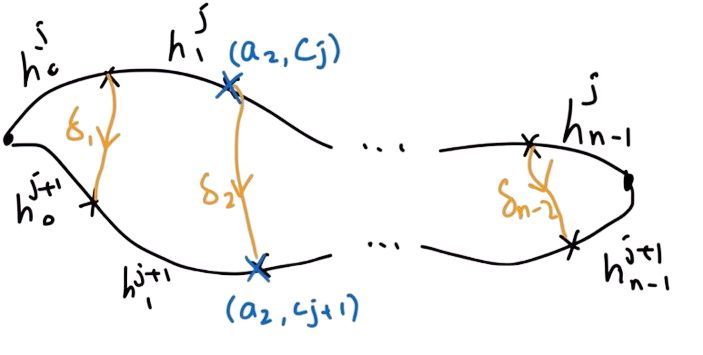
\includegraphics[scale = 0.3]{Image 1}
\end{center}

Now we have that 
\begin{align*}
u([h^j])&=u([h_{n-1}^j])\circ\cdots\circ u([h_0^j])\\
&=u([h_{n-1}^{j+1}\circ\delta_{n-2}])\circ u([\overline{\delta_{n-2}}\circ h_{n-2}^{j+1}\circ\delta_{n-3}])\circ\cdots\circ u([\overline{\delta_1}\circ h_0^{j+1}])\\
&=u([h_{n-1}^{j+1}])\circ\cdots\circ u([h_0^{j+1}])\\
&=u([h^{j+1}])
\end{align*}
By induction, we conclude that $$u([\alpha])=u([h^0])=u([h^1])=\dots=u([h^k])=u([\beta])$$~\\

Now suppose that $A\subseteq X$. By the above lemma, it is sufficient to show that the square for $A$ is a retract of the square for $X$. Let $x\in U\cap V$ and $a_x\in A\cap U\cap V$ lying in the same path component as $x$. Choose a path $\alpha_x:I\to X$ from $a_x$ to $x$ with $\alpha_x$ being constant if $x\in A$. Do a similar choice for $x\in U\setminus(U\cap V)$ and $x\in V\setminus(U\cap V)$. Define $p_{U\cap V}:\Pi_1(U\cap V)\to\Pi_1(U\cap V)[U\cap V\cap A]$ defined by $x\mapsto a_x$ on objects and $$[x\overset{\alpha}{\to} y]\mapsto\left(a_x\overset{[\alpha_x]}{\to}x\overset{[\alpha]}{\to}y\overset{[\alpha_y]}{\to}a_y\right)$$ and similarly for $p_U$ and $p_V$. This defines the natural transformation $p$ in lemma 5.3.4. We conclude by lemma 5.3.4. 
\end{proof}
\end{thm}

Take $A=\{x_0\}$ be a single point in $U\cap V$. Then this theorem shows that there is a pushout diagram \\~\\
\adjustbox{scale=1.0,center}{\begin{tikzcd}
	{\pi_1(U\cap V,x_0)} & {\pi_1(U,x_0)} \\
	{\pi_1(V,x_0)} & {\pi_1(X,x_0)}
	\arrow[from=1-1, to=1-2]
	\arrow[from=1-1, to=2-1]
	\arrow[from=1-2, to=2-2]
	\arrow[from=2-1, to=2-2]
\end{tikzcd}}\\~\\
in $\bold{Grp}$, provided that $A$ contains every path connected component of $U,V,X$. But $A$ is just one point so the condition becomes that $U,V,X$ and $U\cap V$ being path connected. Hence we recover the usual Seifert-Van Kampen theorem in Algebraic Topology 1. 








\end{document}
